%!TEX root = ../thesis.tex
%*******************************************************************************
%****************************** Third Chapter **********************************
%*******************************************************************************
\chapter{The dynamic sRNA profile and inheritance of paternal epigenetic modifications post-fertilisation in the embryo of \textit{Marchantia polymorpha}}

% **************************** Define Graphics Path **************************
\ifpdf
    \graphicspath{{Chapter3/Figs/Raster/}{Chapter3/Figs/PDF/}{Chapter3/Figs/}}
\else
    \graphicspath{{Chapter3/Figs/Vector/}{Chapter3/Figs/}}
\fi


\section{Abstract}

\section{Introduction}

Recently, our group has shown that during spermatogenesis, there extensive DNA methylation reprogramming in Marchantia. As well as the deposition of 5-methylcytosine (5mC), there is an additional wave of DNA methylation reprogramming whereby N4-methylcytosine (4mC) - an epigenetic modification previously only found in prokaryotes – is deposited at the majority of CG cites across the genome \citep{RN189}. 

Data from mature embryo reveals that this 4mC methylation is not present. Several hypotheses could explain why this happens. The most likely is that following fertilisation, paternal epigenetic marks are lost passively through cell division. Alternatively, the marks could be maintained through the first few cell divisions and then are actively or passively lost. We also know that the pronuclei take 3 days to fuse \citep{RN139}, so it is also possible that removing paternal epigenetic marks is required for zygote formation. 

Therefore, my project here will help complement the work that has already been done on 4mC methylation in Marchantia; please see our lab’s preprint for other details of this project \citep{RN189}. Namely, I have already managed to isolate and image embryos 12 days after fertilisation (DAF), and I plan to isolate and stage embryos that are as young as possible to make sure that we can detect 4mC signals if paternal epigenetic marks are maintained through zygote formation but are passively lost during cell division.

\subsection{Overview of DNA methylation in the germline of Marchantia polymorpha}

Recently, our group has shown that during Marchantia spermiogenesis extensive DNA methylation reprogramming occurs. As well as the deposition of 5-methylcytosine (5mC), there is an additional wave of DNA methylation reprogramming whereby N4-methylcytosine (4mC) – an epigenetic modification previously only found in prokaryotes – is deposited at the majority of CG cites across the genome \citep{RN189}.

However, this methylation is absent in the mature embryo (containing over 1000 cells). The exact point in time when 4mC methylation disappears post-fertilisation remains unknown, as does whether the paternal genome retains any 4mC marks during the early stages of zygotic development. The first division of the zygote in Marchantia takes place around 4 days post-fertilisation1 which suggests that 4mC may be required to be actively removed for pronuclear fusion to occur. This aligns with the observed phenotype where embryos fertilised by Mpdn4mt1 sperm develop more rapidly, though this phenotype needs to be confirmed during early embryonic development. Alternatively, 4mC methylation could be lost passively following fertilisation through dilution by cell division, or actively removed post-fertilisation for DNA replication or cell division to function normally. 4mC may also be crucial in the correct genome dosage/transcriptional activity during early embryonic development. 

In Arabidopsis, 5mC methylation is lost actively to maintain homeostasis of DNA methylation levels through several DNA glycosylases, including ROS1 \citep{RN168}. Therefore, the orthologs of ROS1 in Marchantia, MpROS1a and MpROS1x (located on the female sex chromosome) offer possible candidates for erasing paternal 4mC methylation as they are expressed in the sperm \citep{RN212} and mature eggs/embryos \citep{RN257} respectively.

It has also recently been shown that other epigenetic marks, namely the heterochromatic histone modification H3K27me3 is deposited at the pronuclear stage exclusively on the paternal genome and causes the repression of the paternal genome persisting until the conclusion of embryogenesis \citep{RN160}. In contrast, in mammalian germlines, H3K27me3¬ mediated imprinting is limited to a few loci within the female gamete \citep{RN172}.

Hence, investigating the methylation profiles of early Marchantia embryos during the first zygotic divisions and examining the early developmental phenotype of Mpdn4mt1 mutants will complement our previous work, expanding our understanding of how paternal DNA methylation affects early embryonic development.

\begin{figure}[htbp!] 
\centering    
    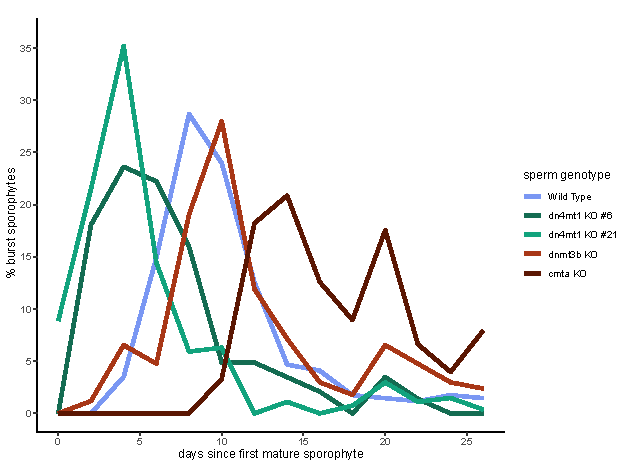
\includegraphics[width=1\textwidth]{Chapter3/Figs/Intro/burstpeak_nuclei_number.pdf}
\caption{\textbf{Embryos fertilised by \textit{dn4mt1} knockout sperm develop more rapidly than WT}}
\label{fig:burstpeak}
\captionsetup{font=small}
    \caption*{Total percentage of burst sporophytes every day since first mature sporophyte, fertilised with wild type sperm (blue), two independent lines of \textit{dn4mt1} knockout sperm (\#6 dark green, \#21 light green) or 5mC (\textit{cmta} (dark brown) or \textit{dnmt3B}) knockout sperm (light brown). }
\end{figure}

\clearpage

\section{Paternal 4mC is lost in the early embryo of \textit{Marchantia}}

To establish an effective method for staging early Marchantia embryos and identify the earliest feasible window for embryo extraction for AMD sequencing, several approaches were explored. Despite incorporating detergents, vacuum-assisted staining, and testing various stains (DAPI, Hoechst 33342, and ethidium bromide), live-cell staining of developing embryos within the archegonium remained inconsistent. This inconsistency likely arises from the embryo's position within a cavity (the venter) surrounded by somatic cells and cell walls (Figure \ref{fig:egg_embryo} rows one and two). Moreover, variations in environmental conditions during embryo development significantly impacted growth, as illustrated in Figure \ref{fig:embryo_diff} which shows the same genotype embryos 10 days post-fertilisation under different growth conditions. To ensure consistency and reproducibility, a controlled crossing method was adopted, wherein archegoniophores were exposed to sperm in a tube for an hour, ensuring synchronised fertilization and uniform embryo development. This approach is particularly suited for studying early embryo development, as embryos can be cultured under these conditions for up to two weeks\citep{RN139}. Under these conditions, the earliest developing embryos could be manually dissected was around 7-8 days after fertilisation (Figure \ref{fig:egg_embryo}).

\begin{figure}[htbp!] 
\centering    
    \includegraphics[width=1\textwidth]{Chapter3/Figs/Figure1_eggs_and_embryos.pdf}
\caption{\textbf{Live cell imaging of the developmental stages of \textit{M. polymorpha} embryos}}
\label{fig:egg_embryo}
\captionsetup{font=small}
    \caption*{Unstained egg cell (first row), DAPI stained egg cell (second row), and embryos 8 days (third row), and 10 days (fourth row) after fertilisation. Scale bar 10$\mu$m}
\end{figure}

As previously established, 4mC methylation is deposited in the CG context over gene bodies and outside of TEs during spermiogenesis by \textit{DN4MT1} (Figure \ref{fig:ends_analysis}A)\citep{RN189}. Although 5mC methylation across all sequence contexts over TEs increases during germline development, non-CG methylation is specifically deposited during spermiogenesis by \textit{MpCMTa} and \textit{MpDNMT3B} (Figure \ref{fig:ends_analysis}B,D,F)\citep{RN189}.  Additionally, this methylation pattern is deposited and maintained over gene bodies (excluding the transcription start site, TSS), with 4mC serving as the primary methylation mark at the TSS. 

As early embryos are difficult to harvest, first AMD-seq (sequencing specifically 4mC) and EM-seq (sequencing specifically 5mC) was tested on wild type sperm and compared to data previously collected from wild type sperm and \textit{dn4mt1} sperm(Figure \ref{fig:ends_analysis} WT sperm rep2 AMD-seq (light green) and dn4mt1 sperm AMD-seq(grey)). The expected methylation patterns over genes and TEs in the 4mC and 5mC contexts were confirmed by the sperm AMD-seq and EM-seq libraries (Figure \ref{fig:ends_analysis} wild type sperm rep2 AMD-seq(light green), wild type sperm EM-seq(dark brown).) 

\begin{figure}[htbp!] 
\centering    
    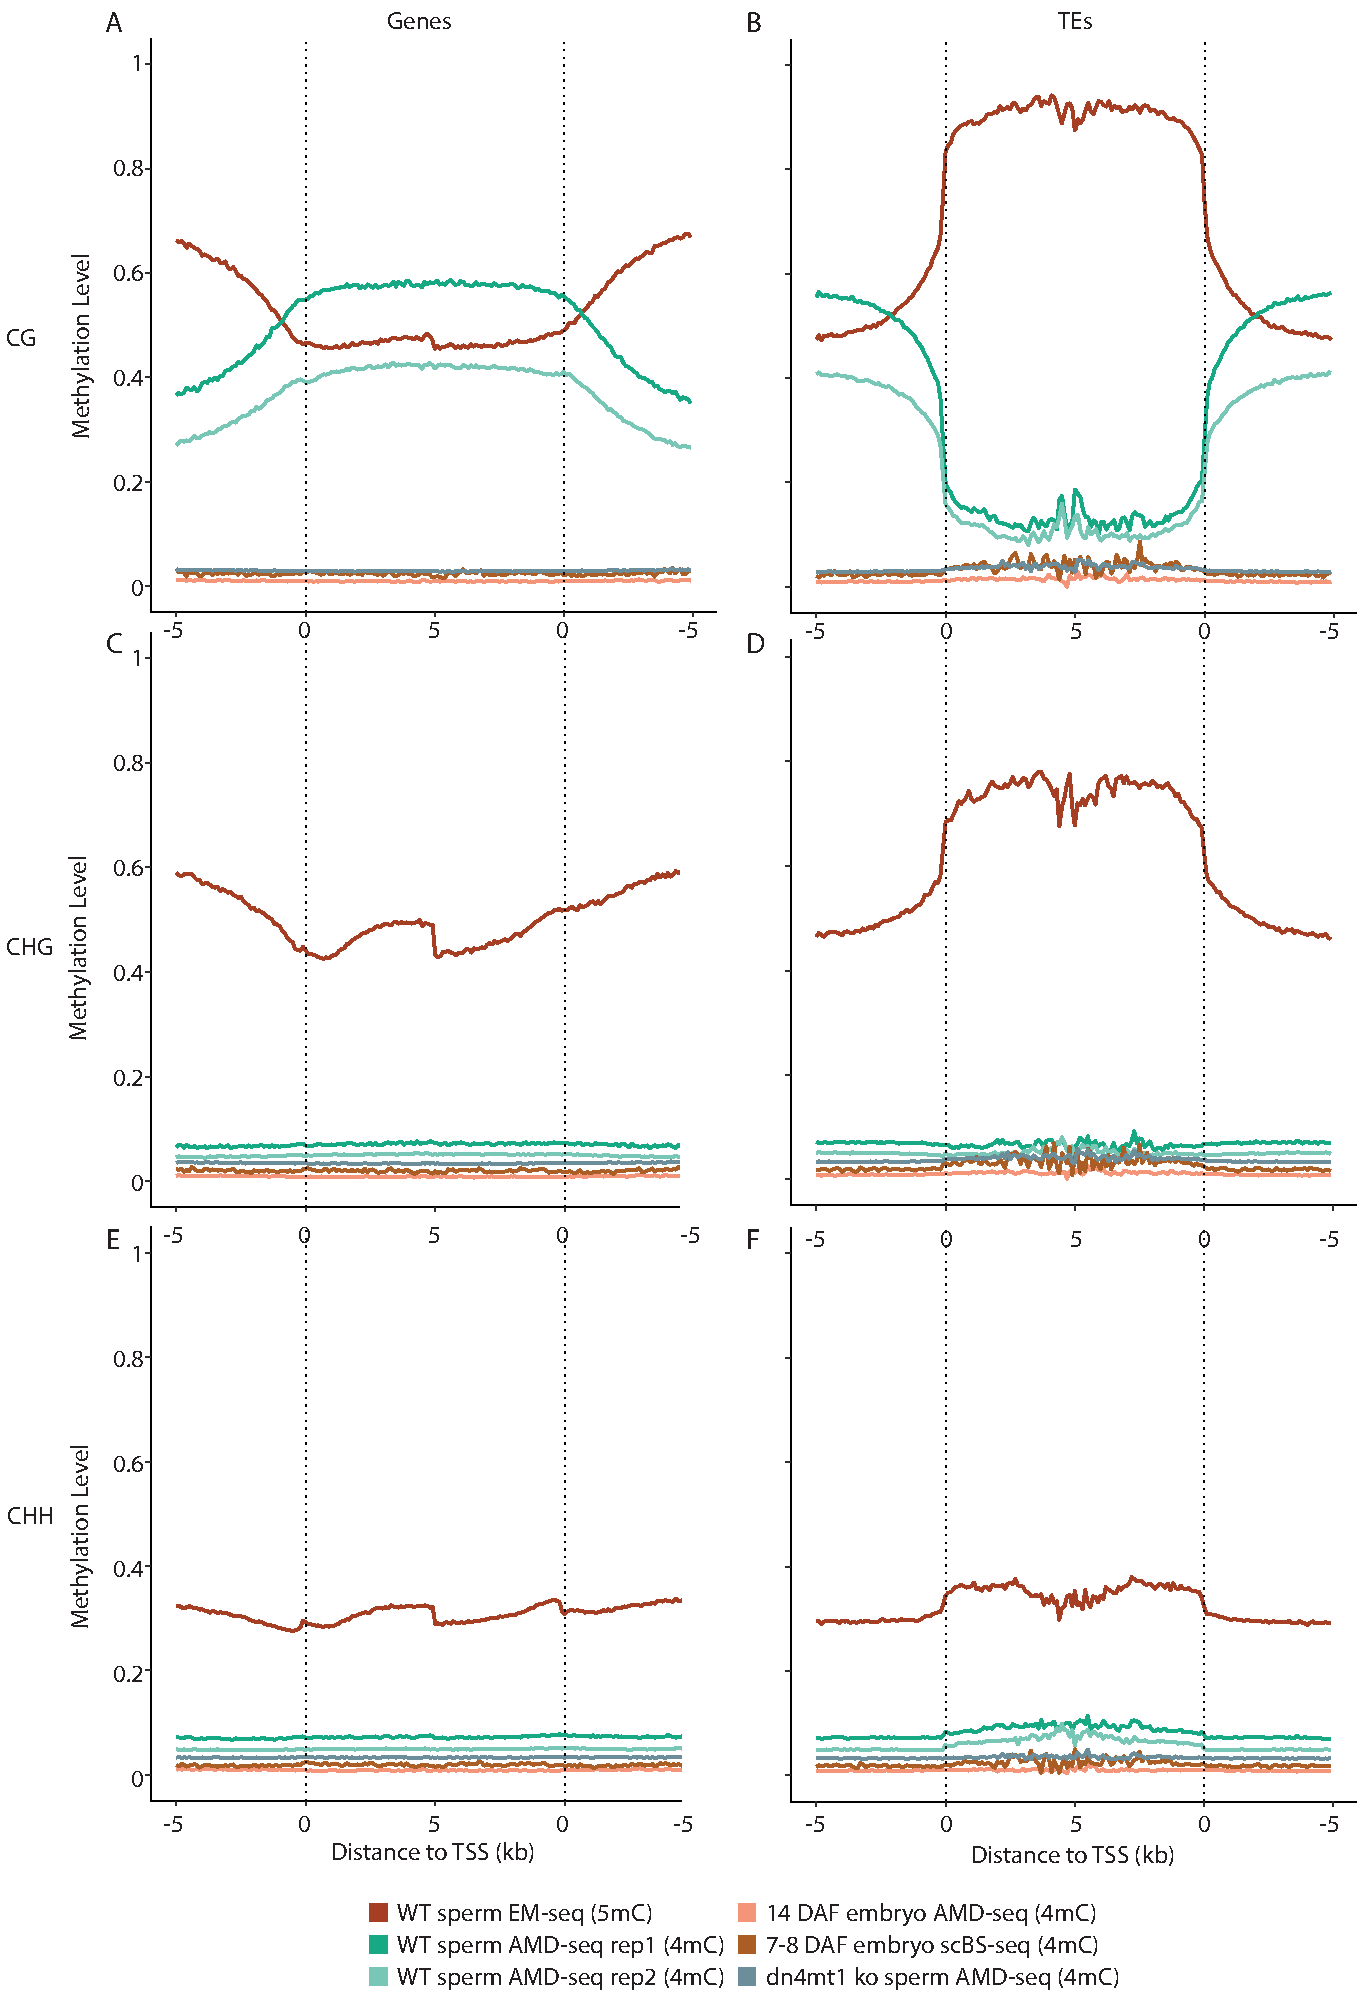
\includegraphics[width=1\textwidth]{Chapter3/Figs/Figure2_ends_analysis.pdf}
\caption{\textbf{4mC methylation occurs in the CG context and is enriched in genic regions and outside of TEs, while 5mC methylation is largerly confined to TEs}}
\label{fig:ends_analysis}
\captionsetup{font=small}
    \caption*{Panel showing 4mC and 5mC methylation across TEs (A) and Genes (B) in CG (first row), CHG (second row) and CHH (third row) sequence contexts in wild type sperm \textit{dn4mt1 sperm}, the embryo 7-8 and 14 days after fertilisation.}
\end{figure}

Secondly, pre-meiotic embryos were dissected and sequenced using AMD-seq to establish a baseline for comparing early embryonic methylation patterns (Figure \ref{fig:ends_analysis}, 14 DAF embryos (orange)). The results confirmed the absence of 4mC methylation over genes or outside TEs (Table \ref{tab:methylation_levels}). Subsequently, 300 embryos at 7–8 DAF were collected, with 200 used for AMD sequencing library construction and the remaining 100 embryos used for bisulfite sequencing libraries, pre-treated with APOBEC3A for an alternative 4mC sequencing method. Although AMD-seq is theoretically capable of handling low DNA input down to picogram levels\citep{idtdna_methylseq_kit}, this was not tested prior to sequencing the early embryos.The bisulfite sequencing protocol, on the other hand, was developed for low-input or single-cell sequencing and this has been robustly tested in our lab. Due to conversion issues, the AMD-seq library was not usable in this study. 

\begin{figure}[htbp!] 
\centering    
    \includegraphics[width=1\textwidth]{Chapter3/Figs/Figure3_H3K27me3.pdf}
\caption{\textbf{H3K27me3 levels are elevated in the paternal genome and correlate with the presence of 5mC over genes}}
\label{fig:h3k27me3}
\captionsetup{font=small}
    \caption*{Heatmaps showing the relative H3K27me3 levels in Marchantia embryos over the genes and TEs in the paternal and maternal genomes.}
\end{figure}

At a surface level, the early embryo AMD-seq data indicated marginally higher 4mC methylation across genes compared to the mature AMD sequencing library (Figure \ref{tab:methylation_levels}). However, this increase fell within the error range of the experimental limitations (Table \ref{tab:methylation_levels}, "CHG and CHH levels of 4mC"). Moreover, the low levels of residual 4mC methylation did not display the expected distribution over genes and TEs, with no relative increase outside TEs or over genes. This suggests that the removal of paternal 4mC methylation may be essential for embryo development. However, starting with a methylation level of around 20\% in the zygote (based on the sperm AMD-seq levels), passive loss of 4mC by the 16–32 cell stage (7–8 days after fertilisation in our conditions) would result in very low residual 4mC methylation levels (Table \ref{tab:methylation_levels}). 

It has been previously demonstrated that during embryonic development the paternal genome is transcriptionally silenced and is marked with the repressive chromatin mark H3K27me3 mediated by maternally expressed Polycomb Repressive Complex 2 (PRC2) in the male pronucleus before the first zygotic division, approximately 3 days after fertilisation \citep{RN160}.  This suggests the existence of a mechanism for paternal genome recognition, with blanket 4mC methylation being a potential candidate. To this end, visualizing H3K27me3 data across genes and TEs from this study confirms a paternal bias in the deposition of H3K27me3. However, the pattern of H3K27me3 occupancy around gene and transposon transcription start sites does not align with the distribution of 4mC. Additionally, Dr. Shujuan Xu confirmed that H3K27me3 paternal foci still form in embryos fertilized by \textit{dn4mt1} knockout sperm, 13 days after fertilisation \ref{fig:immuno}. These findings suggest that paternal genome recognition is not directly linked to blanket 4mC methylation. To obtain a definitive answer, developing reliable 4mC immunostaining and/or single-cell AMD sequencing methods for the zygote or early embryo is necessary, provided successful dissection at this developmental stage is achievable.

\begin{table}[htbp!]
\centering
\captionsetup{font=small}
\begin{tabular}{|p{5cm}|c|c|c||c|c|c|}
\hline
\multirow{2}{*}{\makecell{Methylation context}} & \multicolumn{3}{c||}{Overall} & \multicolumn{3}{c|}{Genes} \\
\cline{2-7}
 & CG & CHG & CHH & CG & CHG & CHH \\
\hline
WT sperm AMD seq rep1 & 0.467 & 0.071 & 0.075 & 0.559 & 0.071 & 0.072 \\
WT sperm AMD seq rep2 & 0.341 & 0.050 & 0.051 & 0.404 & 0.051 & 0.049 \\
dn4mt1 ko sperm & 0.031 & 0.035 & 0.033 & 0.029 & 0.034 & 0.033 \\
14 DAF embryo & 0.011 & 0.009 & 0.009 & 0.009 & 0.008 & 0.008 \\
7-8 DAF embryo & 0.027 & 0.021 & 0.019 & 0.025 & 0.020 & 0.020 \\
\hline
\multicolumn{7}{|l|}{Theoretical methylation levels} \\
\hline
Zygote & 0.202 & 0.030 & 0.031 & 0.241 & 0.030 & 0.030 \\
16 cell embryo  & 0.013 & 0.016 & 0.015 & 0.015 & 0.015 & 0.015 \\
32 cell embryo & 0.006 & 0.007 & 0.007 & 0.008 & 0.007 & 0.007 \\
\hline
\end{tabular}
\caption{\textbf{Methylation levels across WT sperm, \textit{dn4mt1} sperm and the early embryo}}
\label{tab:methylation_levels}
\end{table}


\section{\textit{De novo} methylation is deposited in genic regions specifically in the sporophyte of \textit{Marchantia}, targeted for methylation 24nt sRNAs through mismatches}

As described previously, \textit{de novo} metylation of genes in \textit{Arabidopsis} male meiocytes is mediated by 24nt sRNAs produced by HyperTE loci in the tapetum, the biogenesis of which is iven by CLSY3 chromatin remodeller. Gene body methylation also exists specifically in the embryo and sporophyte of \textit{Marchantia} (Figure \ref{fig:SLM_examples}, data from Dr. James Walker). Sporophytic non-CG DMRs were determined as described before\citep{jimmythesis} and filtered to yield 221 metylated genic loci (MetGenes).

\begin{figure}[htbp!] 
\centering    
    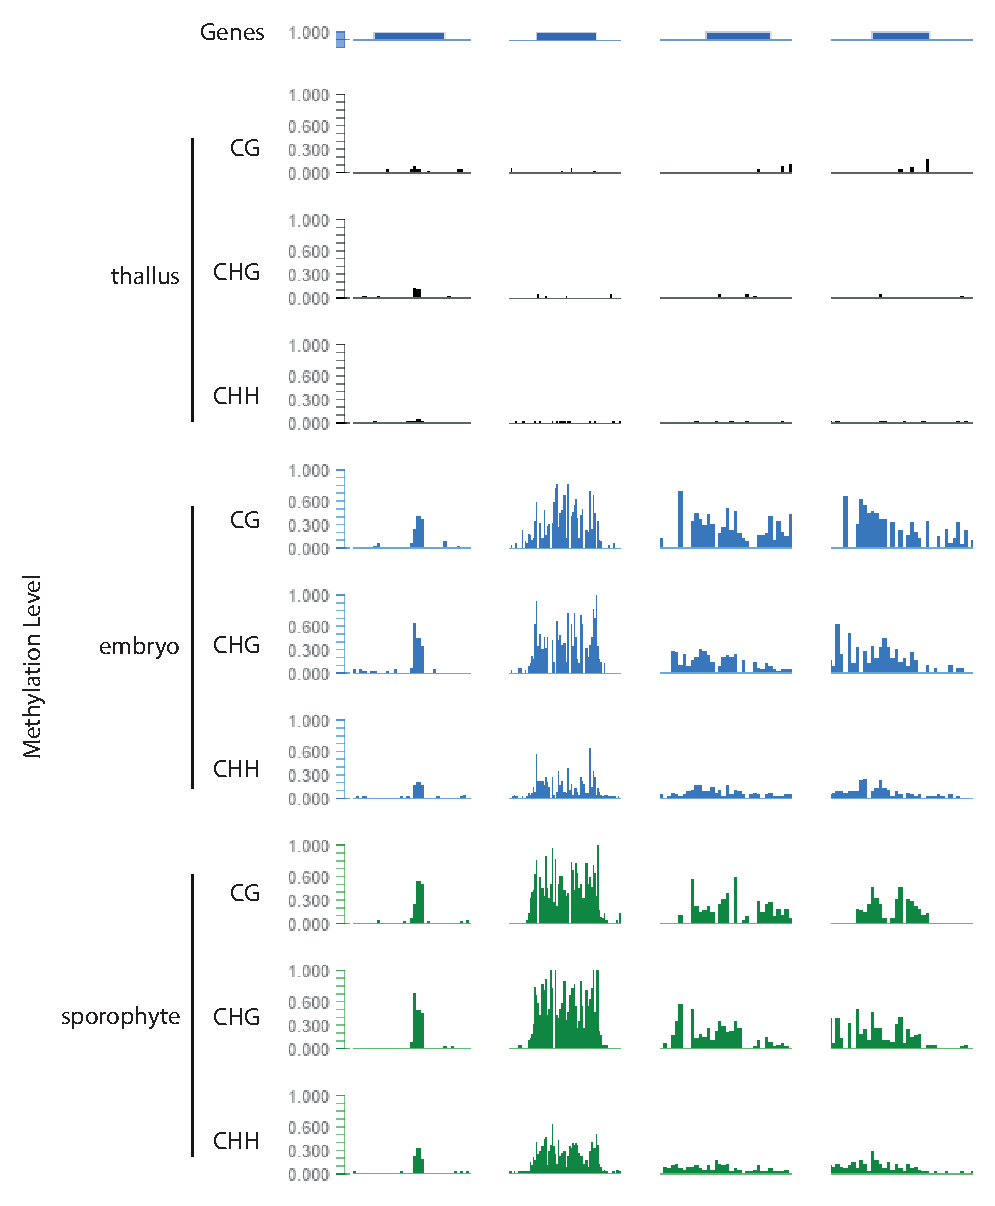
\includegraphics[width=1\textwidth]{Chapter3/Figs/Figure4_SLM_examples.pdf}
\caption{\textbf{Sporophyte specific methylation exists in the embryos of \textit{Marchantia}}}
\label{fig:SLM_examples}
\captionsetup{font=small}
    \caption*{}
\end{figure}

With access to sRNA sequencing libraries from thallus, embryo, and sporophyte, the next step was to determine whether MetGenes could be targeted for methylation through mismatch targeting. To investigate this, the sRNA libraries were mapped to the reference genome allowing for 0 and 3 mismatches. The sRNAs from the 3 mismatch dataset were then remapped onto the 0 mismatch dataset to identify identical sRNA sequences capable of targeting both TEs and genes with up to 3 mismatches. Reads overlapping MetGenes with 3 mismatches and TEs with 0 mismatches were then extracted. The resulting TE-MetGene pairs are visualised in Figure \ref{fig:SLM_targeting}A. It must be noted that one limitation of this method is the challenge of obtaining a comprehensive TE annotation for the gene model used in the study, as not all MetGenes could be paired with annotated TEs.

Indeed when aligning the sequence of a source TE to its corresponding MetGene, an almost perfectly matching \~160bp sequence was found (Figure \ref{fig:SLM_targeting}B). Notably, this alignment corresponds to the exact location where sporophyte-specific methylation is deposited within the MetGene (Figure \ref{fig:TE_SLM_pairs}).

\begin{figure}[htbp!] 
\centering    
    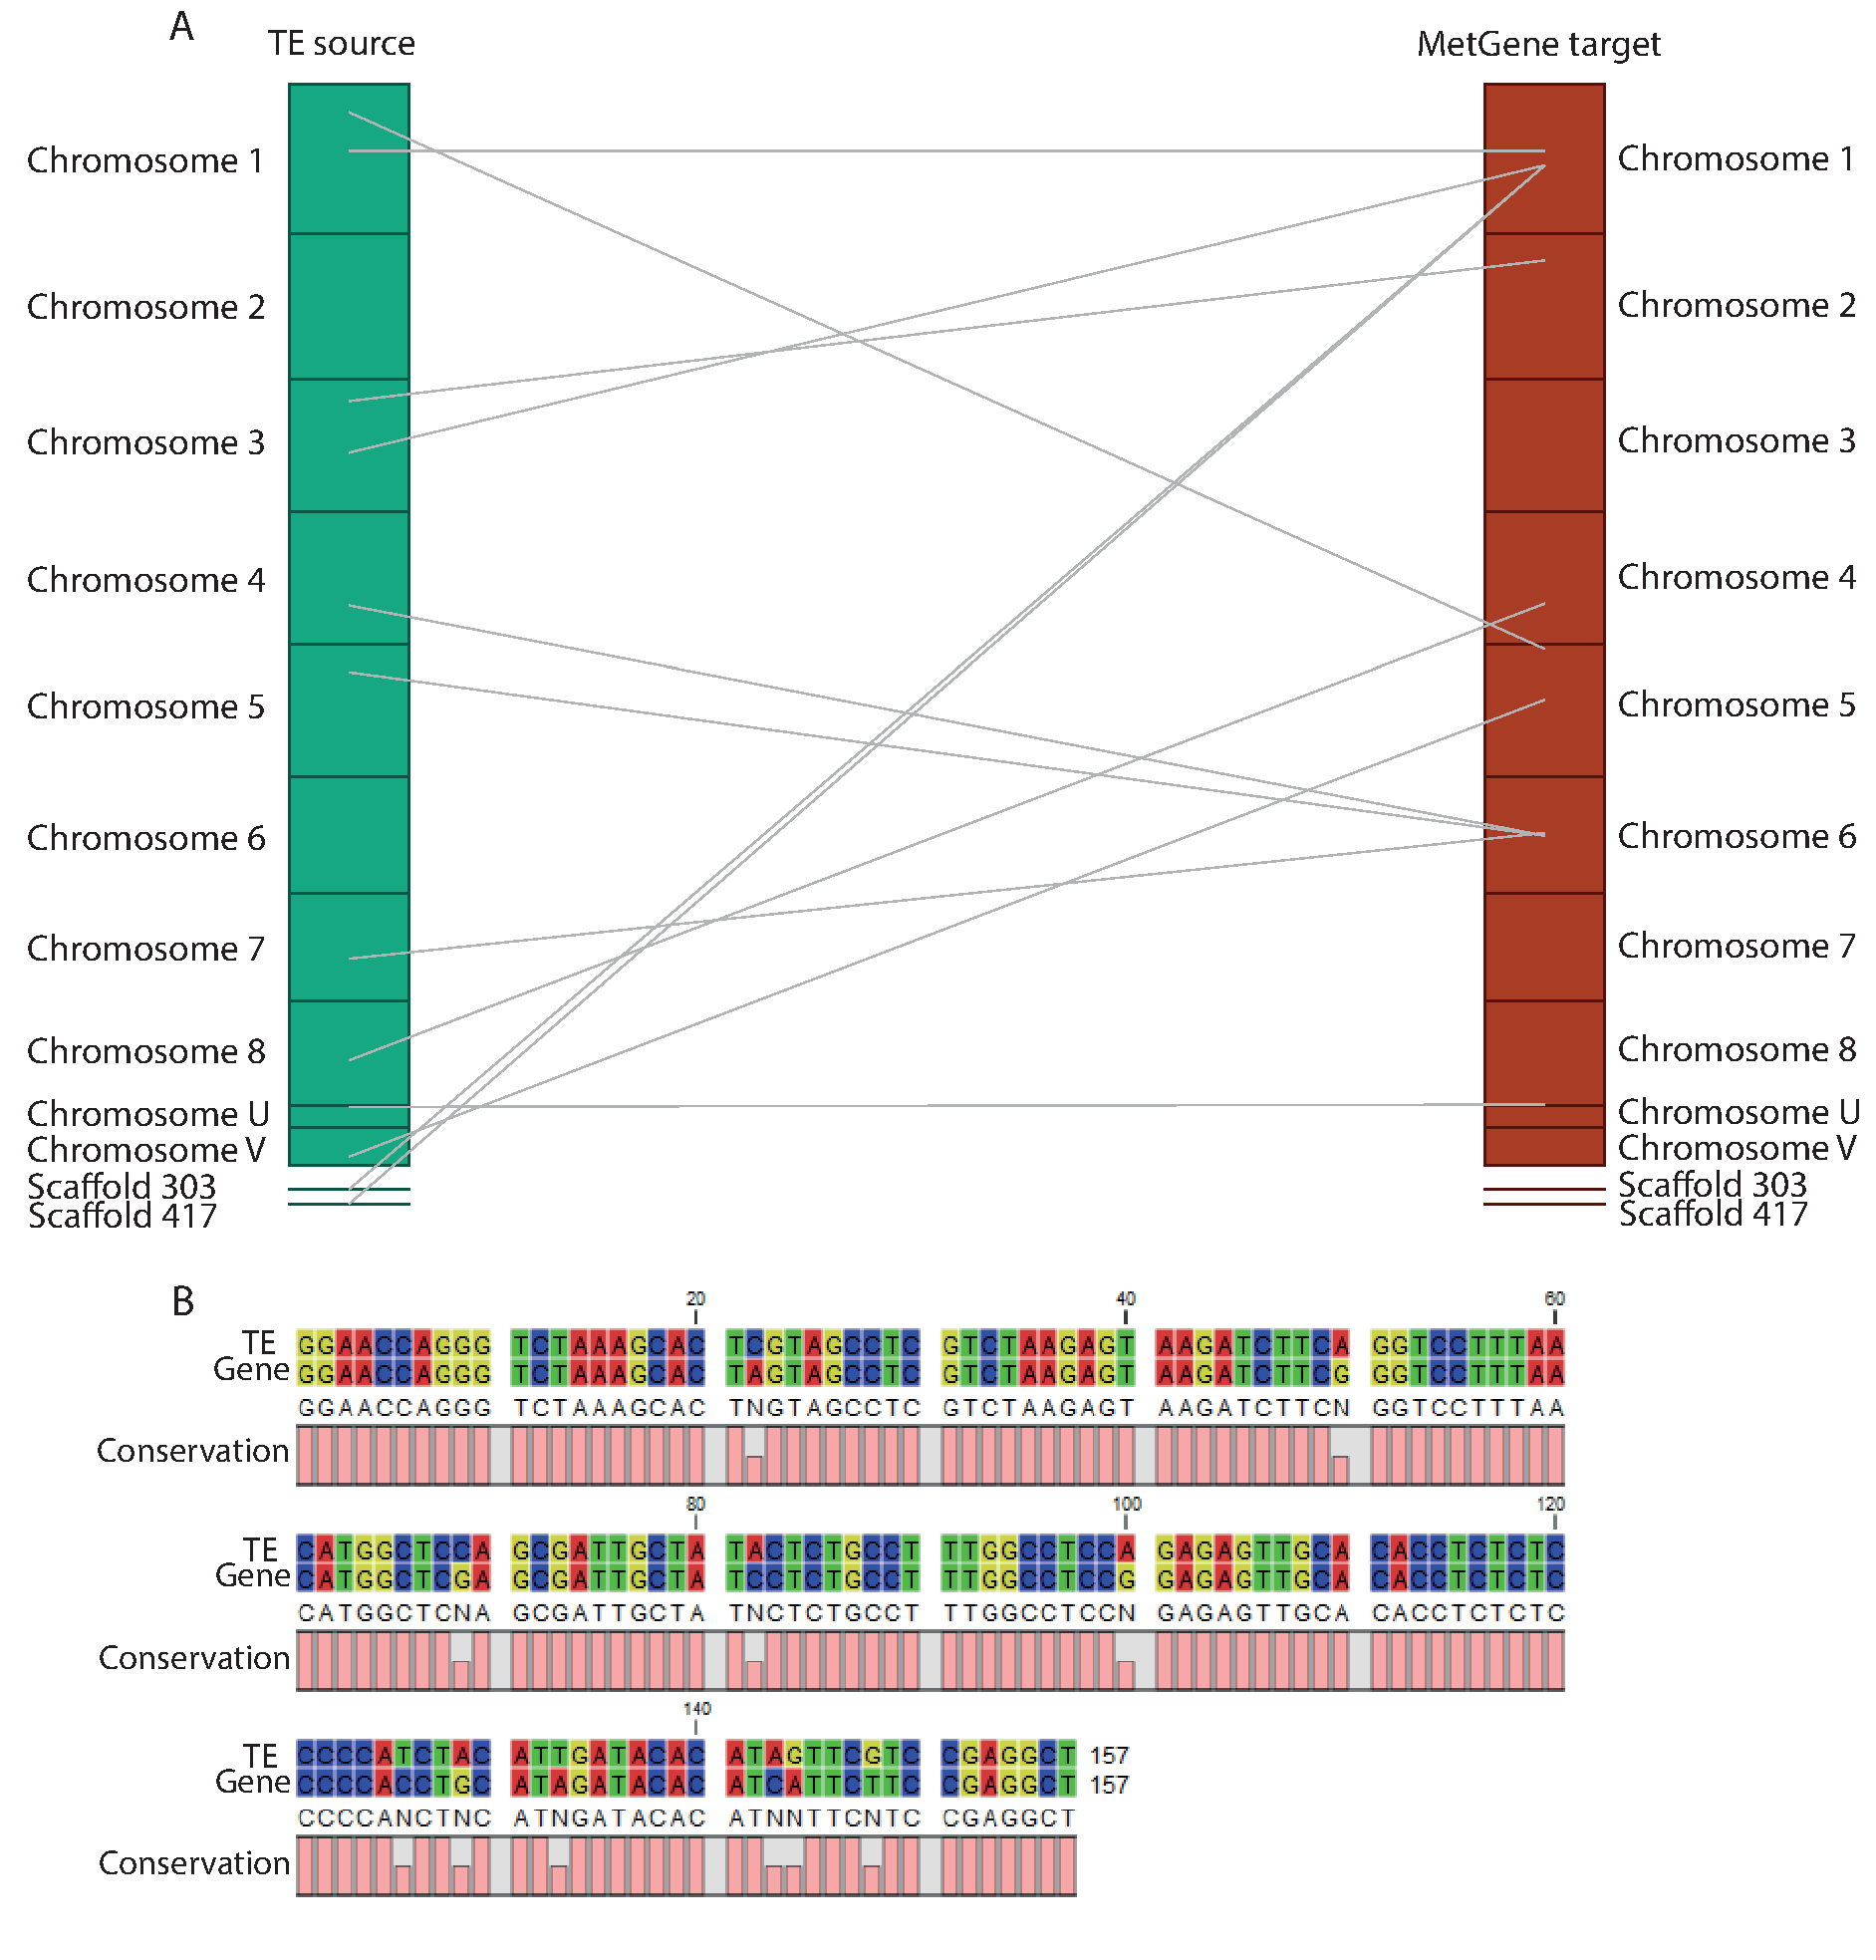
\includegraphics[width=1\textwidth]{Chapter3/Figs/Figure5_SLM_source_target.pdf}
\caption{\textbf{TE loci produce 24nt sRNA that target genic loci for methylation with mismatch targeting}}
\label{fig:SLM_targeting}
\captionsetup{font=small}
    \caption*{Locations of TE source loci (left, green) connected to genic target loci (right, brown)}
\end{figure}

\begin{figure}[htbp!] 
\centering    
    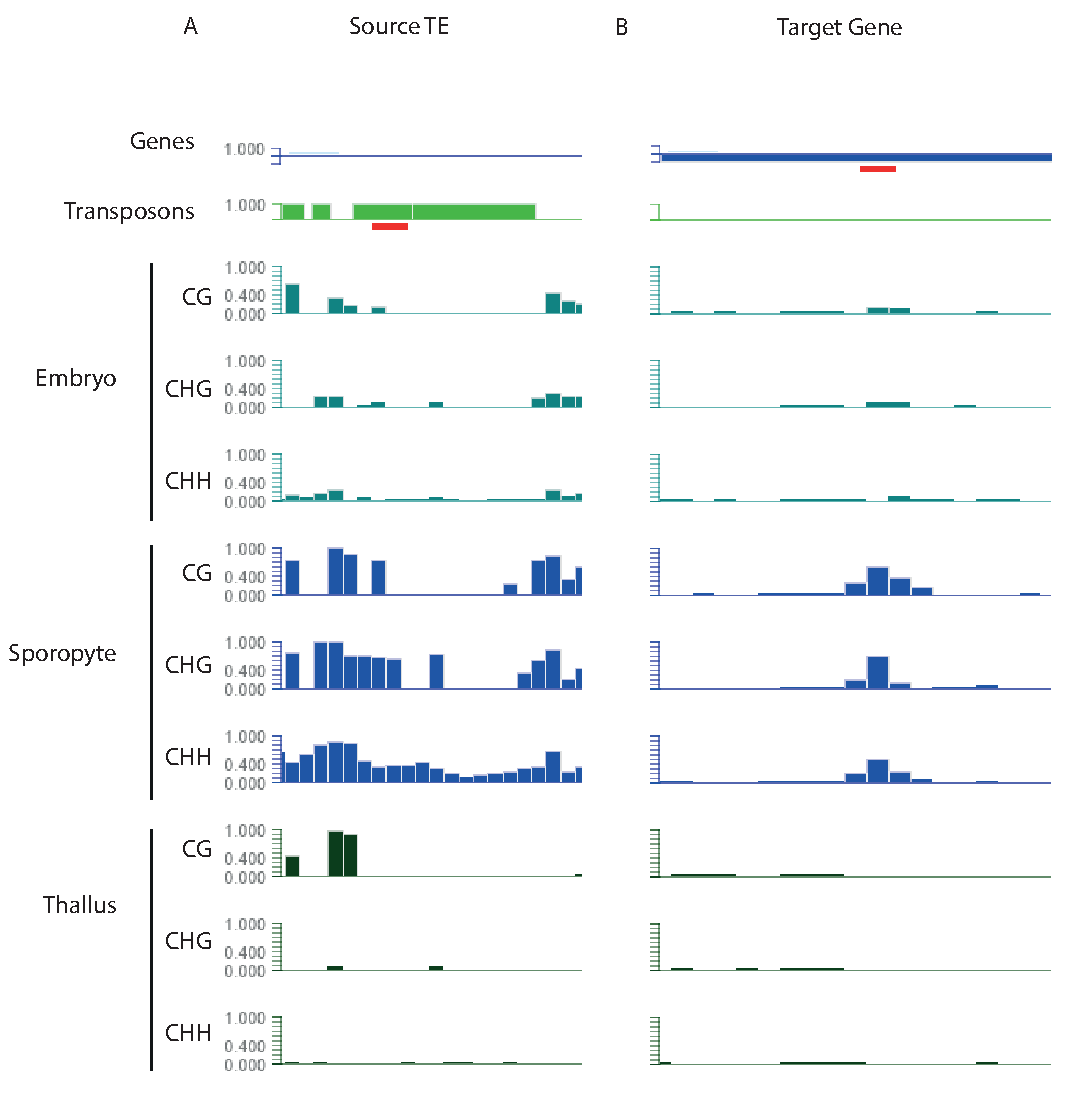
\includegraphics[width=1\textwidth]{Chapter3/Figs/Figure6_pairs_examples.pdf}
\caption{\textbf{Example of a TE  source and SLM target that gain methylation in the sporophyte}}
\label{fig:TE_SLM_pairs}
\captionsetup{font=small}
    \caption*{Methylation levels in (A) TE source and (B) SLM target pair in CG, CHG and CHH sequence contexts in embryo, sporophyte and thallus.}
\end{figure}

\section{Investigating the parental bias of sRNA production in \textit{Marchantia} embryos, sporophyte and thallus}

In the developing embryo, the paternal genome is deposited with H3K27me3, resulting in tight heterochromatic foci and transcriptional silencing \citep{RN160}. This raises the question of whether sRNA production in the embryo and sporophyte is biased toward the maternal genome.To explore this, single nucleotide polymorphisms (SNPs) between Tak-1 (male) and Tak-2 (female) were analysed to calculate a SNP ratio. sRNA sequencing libraries utilised from the thallus, archegoniophore, and antheridiophore \citep{RN265} in addition to the libraries previously mentioned.

The sRNA sequencing libraries were mapped to the reference genome with both no mismatches, and allowing one mismatch. Reads with mismatches at SNP positions were retained, as well as perfect matching sRNAs at SNP positions. A SNP ratio was calculated between the alternative and reference alleles for further analysis. Although several thousand SNP regions were initially covered, only those with at least 5 reads were retained to ensure robust results, which substantially reduced the number of SNP locations. 

Reads from archegoniophores displayed a SNP ratio near 1, as expected (Figure \ref{fig:sRNA_SNPs}A,B archegoniophore). Interestingly, in the early embryo, the data suggest a paternal bias in sRNA production, which shifts to a maternal bias in the sporophyte (Figure \ref{fig:sRNA_sizes}A,B embryo and sporophyte). As expected, the SNP ratio distribution in the embryo and sporophyte was less bimodal than in other tissues, indicating concurrent sRNA production from both genomes at multiple loci in the diploid phase. The thallus data seemed unreliable, with a surprising maternal bias despite originating from Tak-1 males \citep{RN265}.

It is important to recognise the limitations of these results. Since Tak-1 and Tak-2 are asexually maintained in lab conditions, accumulated point mutations may alter the genomic sequence significantly over time. In fact, at several SNP positions, bases other than the reference or alternative were found, in all datasets. Additionally, if Tak-1 was crossed with other lines at any point, the SNP distribution in the resulting hybrid would differ from either parent. The unequal SNP distribution along different chromosomes also makes these cultivars suboptimal for complete genome coverage. Variations in SNP ratio distribution across chromosomes (Figure \ref{fig:chrom_ridge}) further illustrate this. Lastly, the filtering steps applied to the sRNA data resulted in a limited number of data points, which restricts the ability to draw definitive conclusions. Therefore, ensuring the precise genetic background of the parental lines is crucial for accurate results, as well as obtaining sufficient sequencing depths, especially to determine definitively whether 24nt sRNAs are produced from both parental genomes in \textit{Marchantia} embryo development.

\begin{figure}[htbp!] 
\centering    
    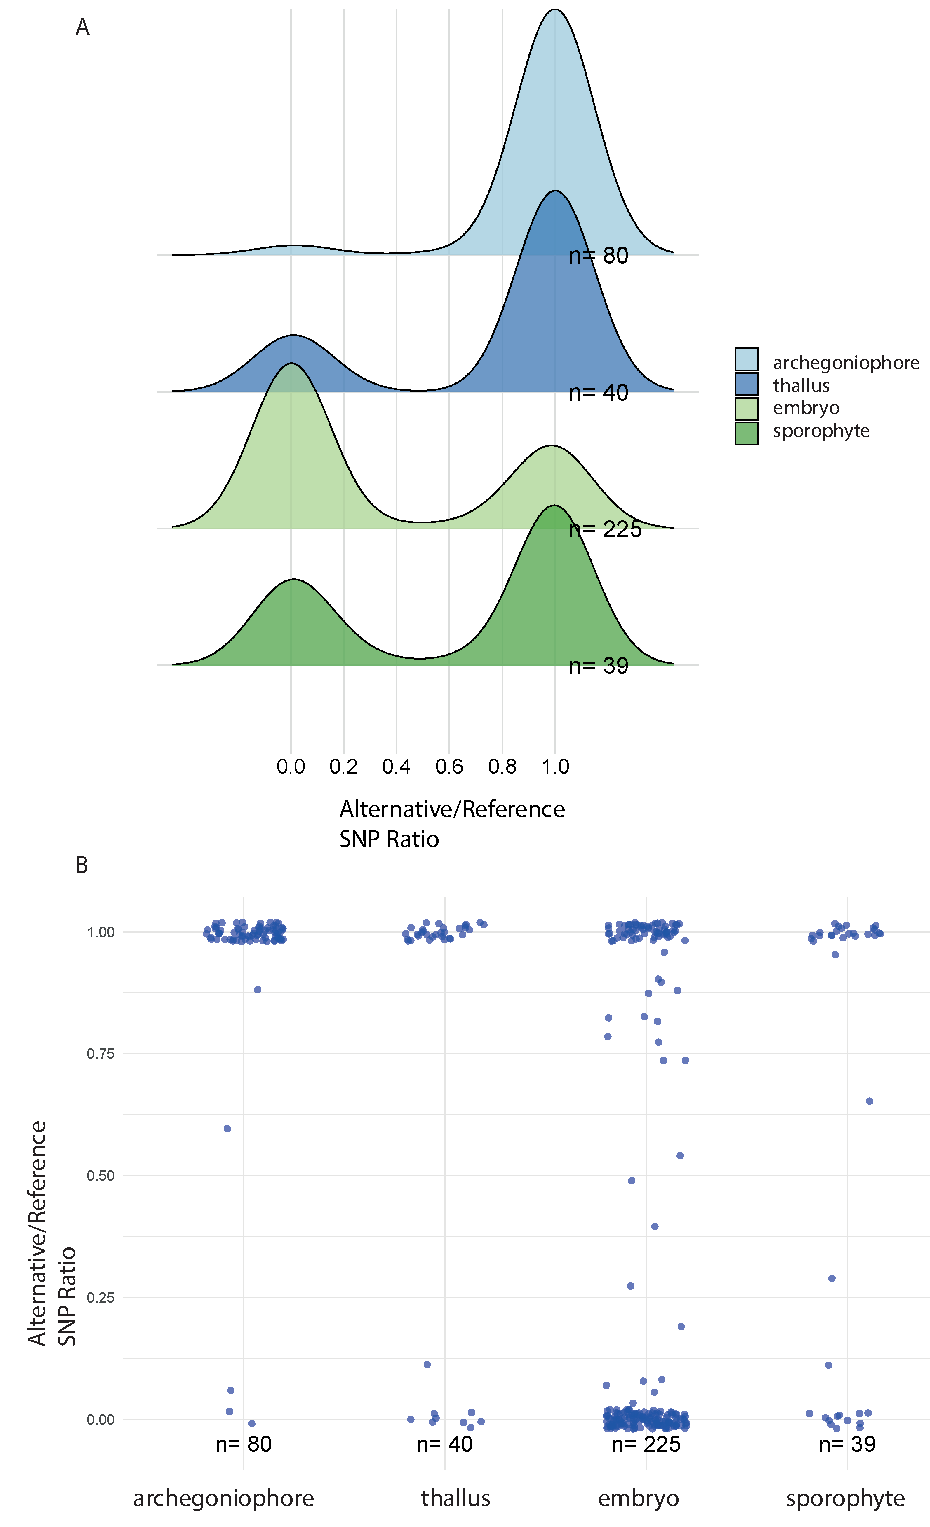
\includegraphics[width=1\textwidth]{Chapter3/Figs/Figure_sRNA_SNPs.pdf}
\caption{\textbf{}}
\label{fig:sRNA_SNPs}
\captionsetup{font=small}
    \caption*{}
\end{figure}

\clearpage

\section{Developing an effective method for visualising early embryonic development in \textit{Marchantia}}

The next objective was to determine whether the observed phenotype — where embryos fertilized with 4mC methylation mutants reach maturity earlier than wild type (Figure \ref{fig:burstpeak}) — was due to accelerated pronuclear fusion in the zygote, potentially caused by the absence of paternal 4mC. This led to the hypothesis that paternal 4mC may need to be actively removed before pronuclear fusion can occur.

As described earlier, staining live \textit{Marchantia} embryos proved challenging. A variety of fixing and staining methods were also trialled, including DAPI, Hoechst 33342 and ethidium bromide as staining dyes (the latter was used due to its small molecule size, which was expected to penetrate the fixed embryo), as well as different triton and paraformaldehyde concentrations and fixation times. Additionally, an egg cell reporter line was also tested (ECpro:MpSUN-GFP \citep{RN139}) showing strong expression;this faded after the first zygotic division, making it insufficient for visualizing early embryonic development (Figure \ref{fig:MpSUN}). 

Next, cell wall digestion enzymes such as cellulase and pectinase were trialed to improve dye penetration. While these enzymes increased dye uptake, they also compromised cell ultrastructure, hindering proper imaging of early embryonic development and cellular ultrastructure (Figure \ref{fig:enzyme_tests}). As a result, four constructs were designed to create constitutively expressing nuclear reporter lines. These constructs were driven by either the constitutive 35S promoter or the native EF$\alpha$ promoter, fused with citrine or tdTomato, and tagged with a nuclear localisation signal (NLS) (Figures \ref{fig:35S_citrine_map}, \ref{fig:35S_tdTomato_map}, \ref{fig:EFalpha_citrine_map}, \ref{fig:EFalpha_tdTomato_map}). 

\begin{figure}[htbp!] 
\centering    
    \includegraphics[width=1\textwidth]{Chapter3/Figs/Figure7_Reporter_line_gemmae_screening.pdf}
\caption{\textbf{Gemmae screening of constitutively expressed nuclear reporter lines}}
\label{fig:gemma:screen}
\captionsetup{font=small}
    \caption*{Nuclear signal of tdTomato or citrine (second column, red or yellow respectively, white arrows) in gemmae, driven by either 35S constitutive promoter (first row) native constitutive promoter EF$\alpha$ (second and third rows). Scale bar 10$\mu$m.}
\end{figure}

The constructs were initially transformed into Tak-1 thalli and selected in gemmae to avoid chimeric expressio, resulting in the recovery of several independent plants from three of the four constructs(Figure \ref{fig:gemma:screen}).The constructs were then also transformed into sporelings from WTxWT, WTx\textit{dn4mt1} \#6 knockout and WTx\textit{dn4mt1} \#21 knockout crosses. Transformants were successfully recovered and screened for fluorescence expression in gemmae and antheridia (Figure \ref{fig:antheridia_screen}). Interestingly, while citrine reporter lines showed strong expression in gemmae, the strongest and most consistent expression was observed in transformants with the 35S::tdTomato-NLS and EF$\alpha$::tdTomato-NLS constructs. These lines were selected for crosses with wild-type female archegonia.

\begin{figure}[htbp!] 
\centering    
    \includegraphics[width=1\textwidth]{Chapter3/Figs/Figure8_Reporter_line_antheridia.pdf}
\caption{\textbf{The tdTomato based nuclear reporter lines are expressed in the antheridia}}
\label{fig:antheridia_screen}
\captionsetup{font=small}
    \caption*{Nuclear signal of tdTomato or citrine (second column, red or green respectively) in the antheridiophore, driven by either 35S constitutive promoter (first row) native constitutive promoter EF$\alpha$ (second and third rows). Scale bar 10$\mu$m.}
\end{figure}

Unfortunately, despite strong expression in the antheridia, no nuclear reporter expression was detected in the developing zygote or embryo.This may be attributed to the previously mentioned shutdown of the paternal genome (Figure \ref{fig:malevsfemale}, first and second rows).  In response to this, wild-type female plants were recovered from the WTxWT 35S::tdTomato-NLS and  EF$\alpha$::tdTomato-NLS sporeling crosses (Figure \ref{fig:malevsfemale}, rows 3 and 4) strongely expression their respective nuclear reporter lines.

\begin{figure}[htbp!] 
\centering    
    \includegraphics[width=1\textwidth]{Chapter3/Figs/Figure9_reporter_line_malevsfemale.pdf}
\caption{\textbf{Tak1 male nuclear reporter lines crossed to Tak2 females have no nuclear expression in the embryo}}
\label{fig:malevsfemale}
\captionsetup{font=small}
    \caption*{Nuclear signal of tdTomato (second column, red, white arrows) in embryos crossing EF$\alpha$::tdTomato-NLS Tak1 male to WT Tak2 female, 3 days (first row) and 16 days (second row) after fertilisation. Expression of EF$\alpha$::tdTomato-NLS (third row) and  35S::tdTomato-NLS (fourth row) in WT female thallus. Scale bar 10$\mu$m.}
\end{figure}

\section{Embryos crossed with 4mC metylation mutant sperm develop more rapidly than wild type during the first 7 days post-fertilisation}

Once mature archegoniophore-producing female plants were available from the selected 35S::tdTomato-NLS and EF$\alpha$::tdTomato-NLS lines, they were crossed with WT, \textit{dn4mt1} \#6 and \textit{dn4mt1} \#21 sperm. As before, the sperm was co-cultured with the archegoniophores for an hour, after which the developing embryos were fixed and cleared daily, 1 to 7 days post-fertilisation. 

\begin{figure}[htbp!] 
\centering    
    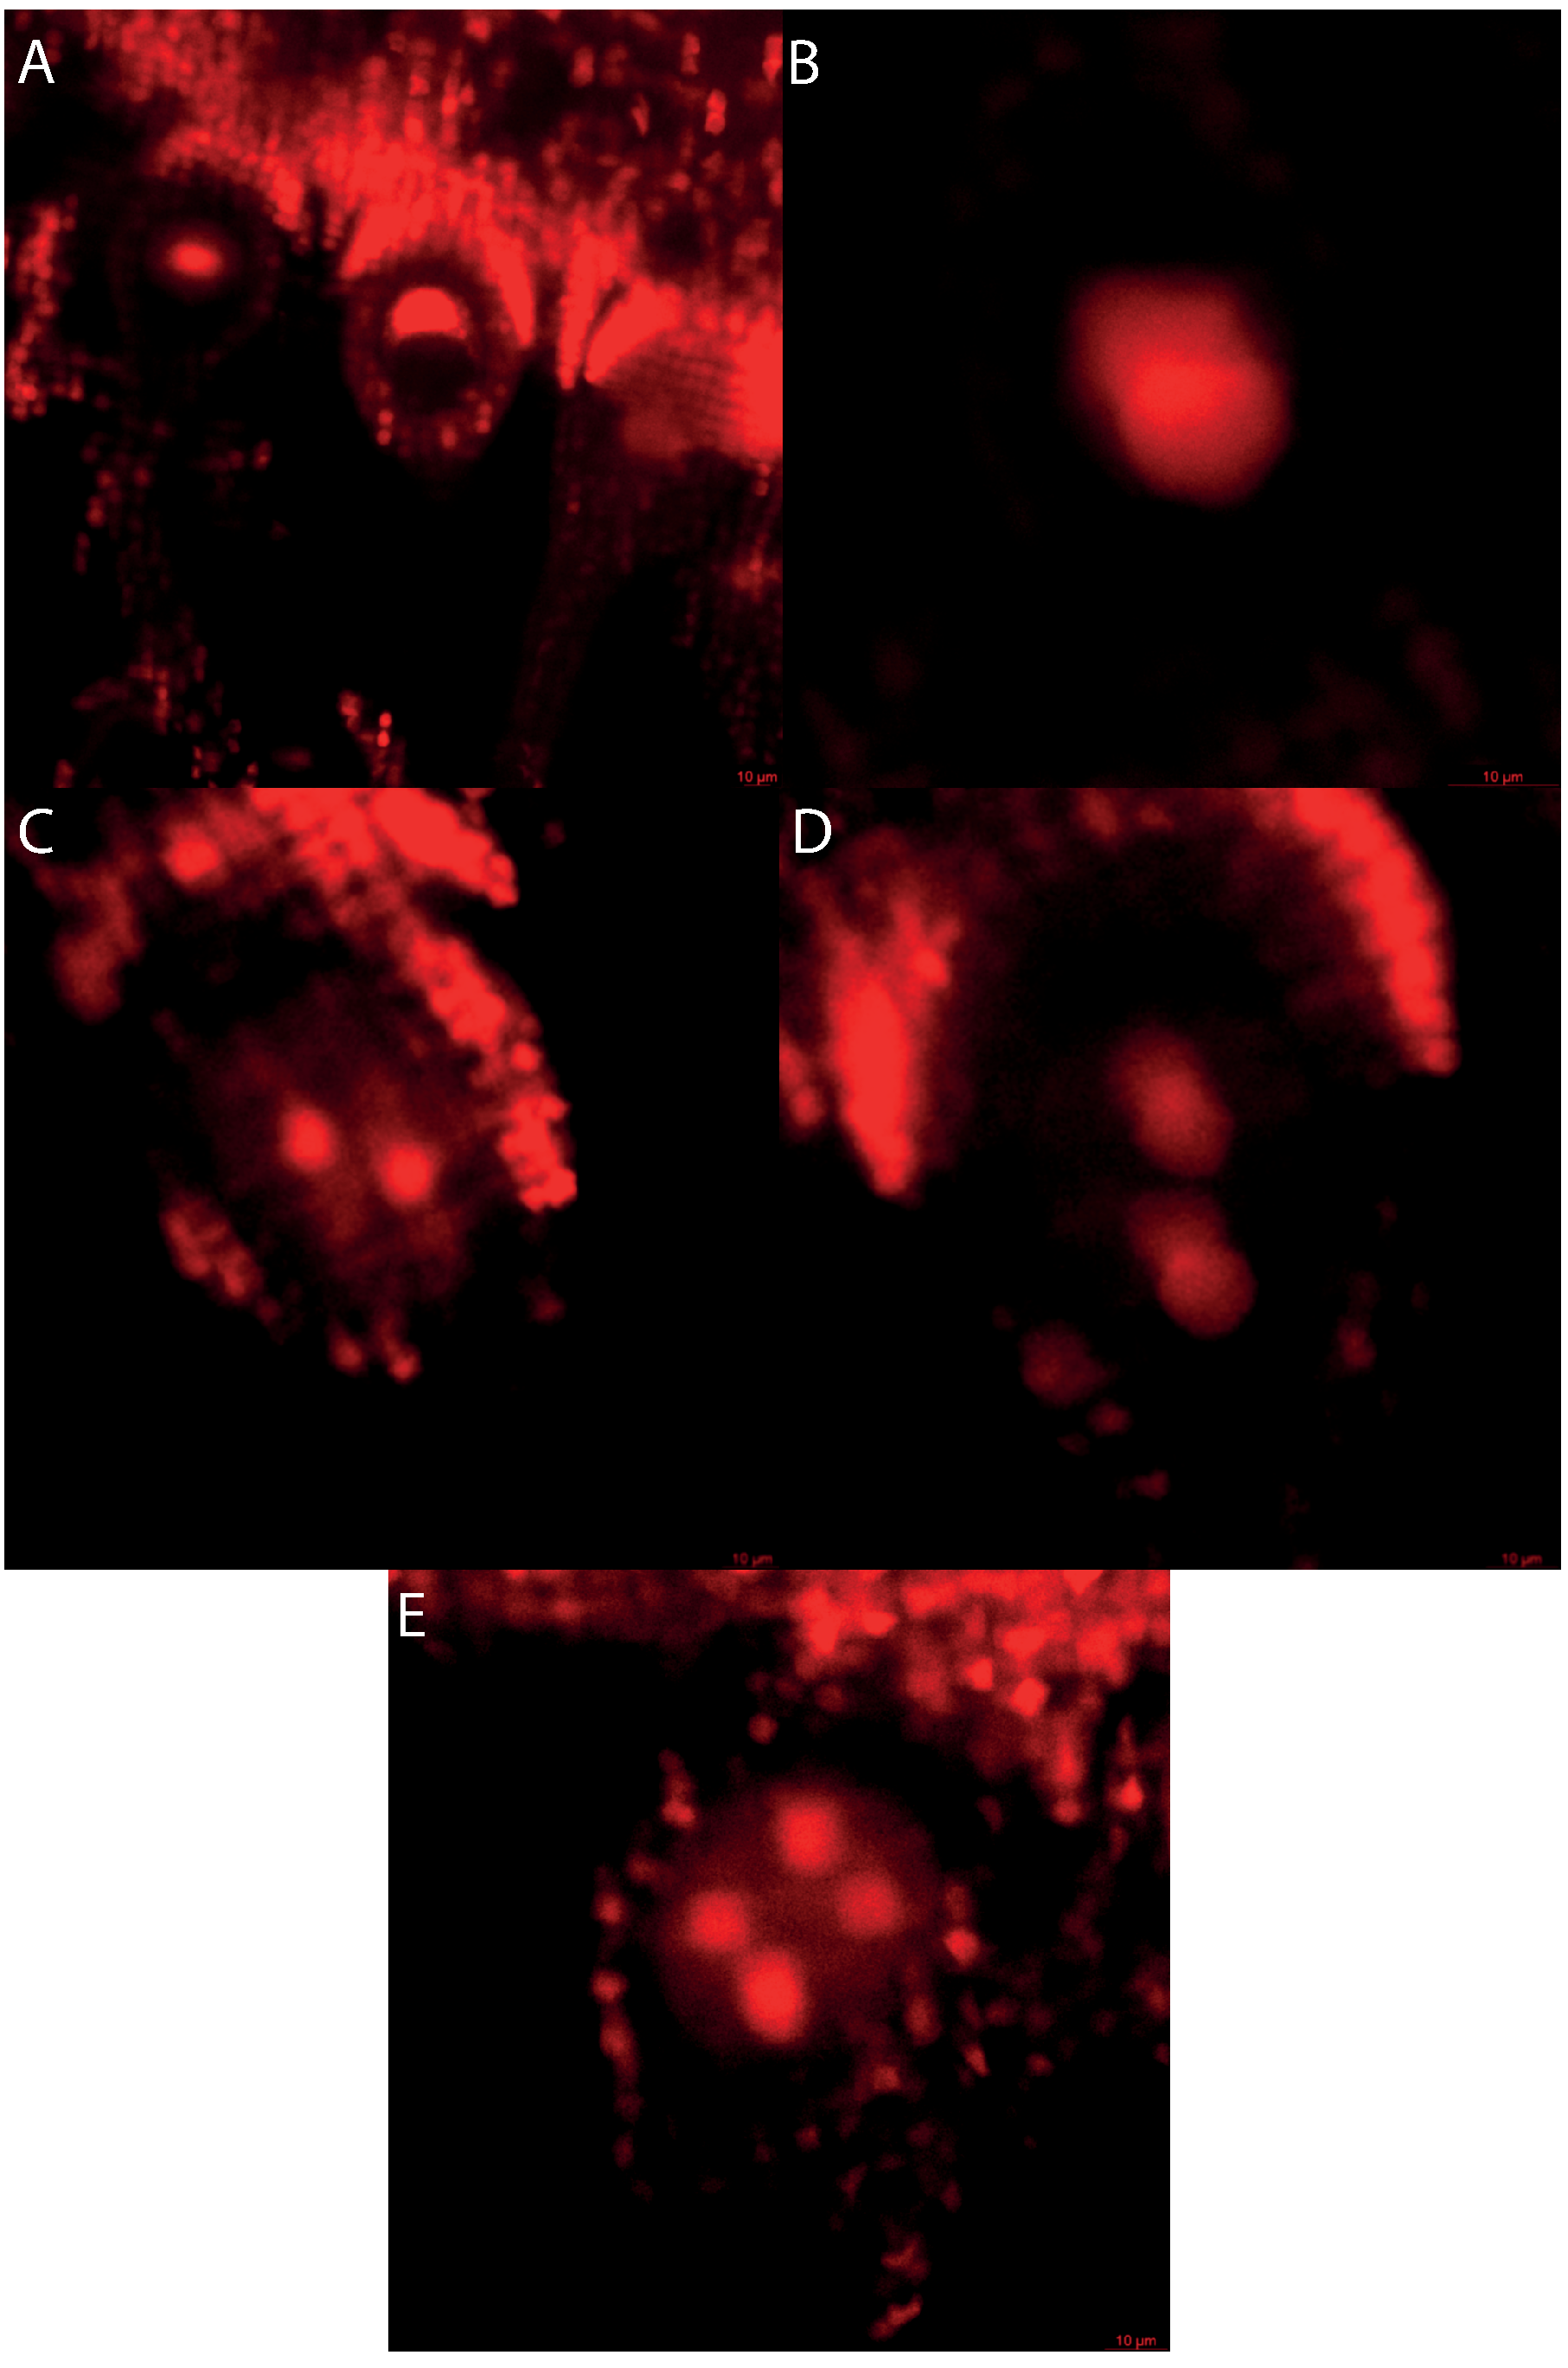
\includegraphics[width=1\textwidth]{Chapter3/Figs/Figure10_Developmental_stages.pdf}
\caption{\textbf{Developmental stages of the early embryo (Tak1 male x EF$\alpha$::tdTomato-NLS WT female)}}
\label{fig:dev_stages}
\captionsetup{font=small}
    \caption*{(A) Zygote (B) Zygote dividing (C) Two-cell stage (D) Two-cell embryo dividing (E) Four-cell stage. Scale bar 10$\mu$m.}
\end{figure}

During the first two zygotic divisions, cells were often observed with multiple nuclei that had not yet undergone cytokinesis (Figure \ref{fig:dev_stages}B and D). Between days 1-5 after fertilisation, embryos fertilised by either independent \textit{dn4mt1} knockout lines appeared to begin dividing earlier than those fertilised by wild type sperm (Figure \ref{fig:nucleus_number}). Interestingly, according to the hypothesis, the task of the removal of the blanket 4mC methylation in the paternal genome should delay pronuclear fusion in wild type zygotes compared to the 4mC knockout mutants, leading to a delayed onset of exponential growth in the developing embryo. However, the results show that up to day 5 post-fertilisation, both WT and 4mC mutants had similar nuclei numbers, despite the earlier zygotic division observed in the 4mC mutants \ref{fig:Dividing_cells}. After day 5, the rate of cell division in 4mC mutants sharply increased, whilst the rate of cell division in wild type showed a less steep gradient (Figure \ref{fig:nucleus_number}).

The developing embryo initially elongates through a transverse division (perpendicular to the archegonial axis), followed by a second vertical division to form four cells. The third division occurs at right angles to the previous divisions, creating an octant of equal cells \citep{RN143,RN144}, after which a series of cell divisions alters the embryo's initially circular shape. Therefore the mean transverse diameter of the developing cavity of the embryonic venter was used to approximate early cellular development. Interestingly, despite the sharp divergence if nucleus number between wild type and the 4mc knockout lines after 5 DAF, the mean transverse diameter of the embryos remained consistent and increased at a similar rate across all lines all until day 6, and between WT and \textit{dn4mt1} k.o. \#6 between days 6 and 7. 


\begin{figure}[htbp!] 
\centering    
    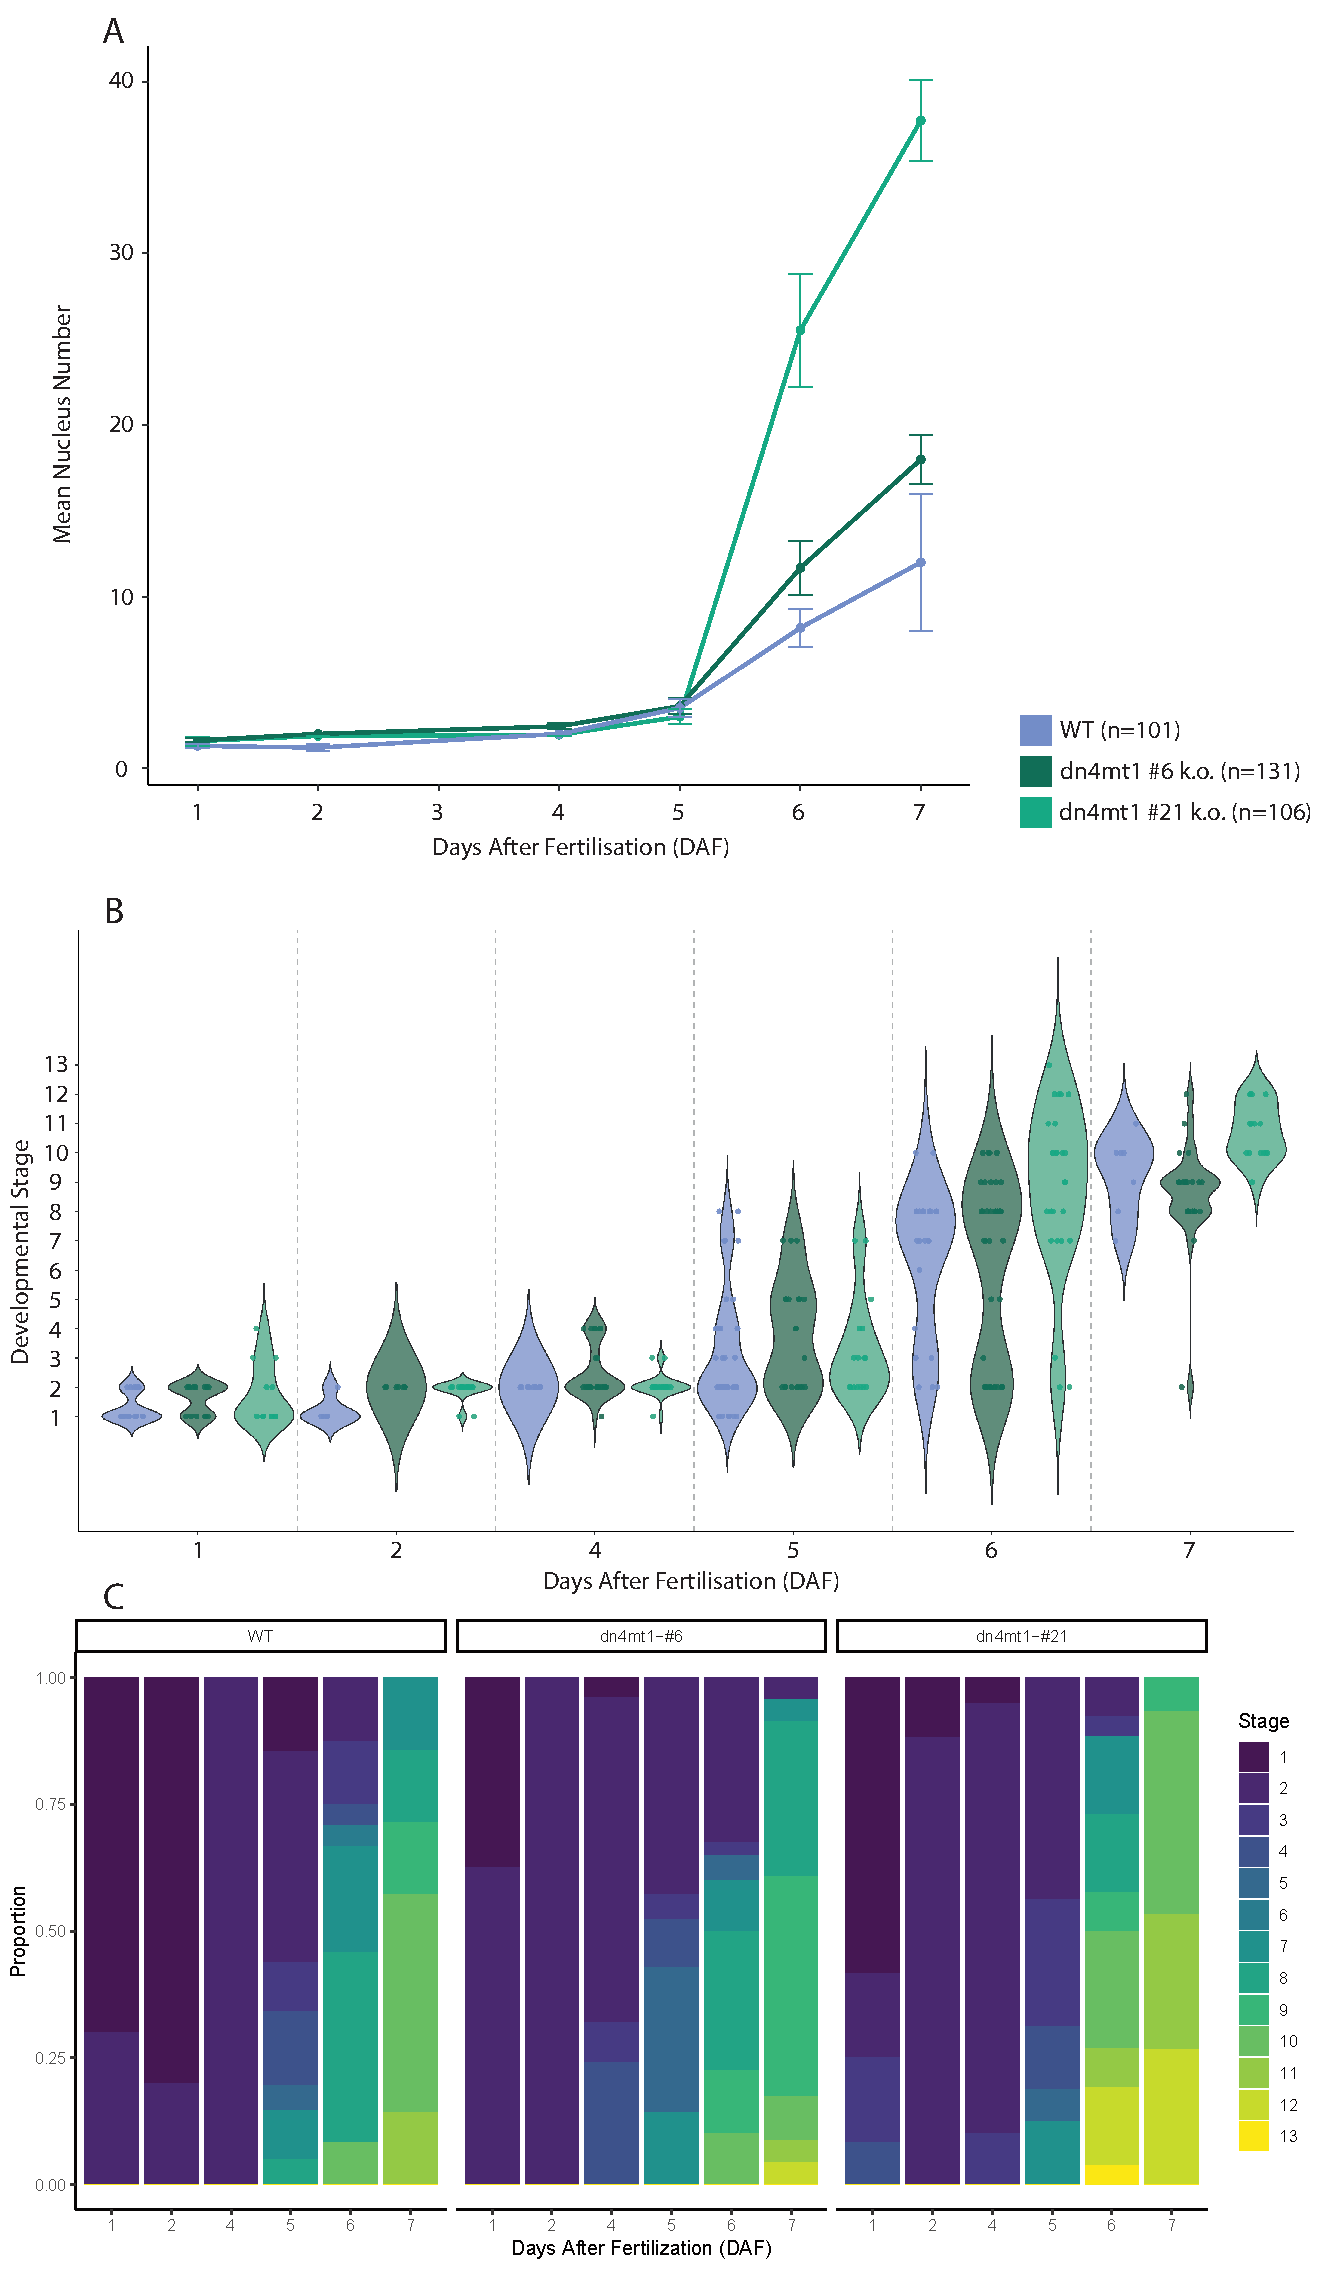
\includegraphics[width=1\textwidth]{Chapter3/Figs/Figure11_nucleus_number.pdf}
\caption{\textbf{Embryos fertilised by \textit{dn4mt1} knockout sperm develop more rapidly than WT}}
\label{fig:nucleus_number}
\captionsetup{font=small}
    \caption*{Mean nucleus number of embryos from 1-7 days after fertilisation, fertilised by wild type (blue), \textit{dn4mt1} knockout \#6 (dark green), or \textit{dn4mt1} knockout \#21 (light green) sperm. }
\end{figure}

\clearpage


\section{Discussion}

In angiosperms and other land plants during spermiogenesis, histones get swapped out to  sperm specific histones. However in Marchantia this is not the case, histone modifications cannot be transferred to the  sperm, instead histones get replaced by protamines, thereby DNA methylation is the only heritable epigenetic modification from the paternal side. This is strikingly similar to mammalian sperm compaction. In addition, after fertilisation the developing zygote is quickly demethylated by TET2 enzymes. In plants, DNA demethylation os carried out by RESPRESSOR OF SILENCING 1 (ROS1) and 

DNA demethylases regulate DNA methylation levels in eukaryotes. Arabidopsis encodes four DNA demethylases, DEMETER (DME), REPRESSOR OF SILENCING 1 (ROS1), DEMETER-LIKE 2 (DML2), and DML3. While DME is involved in maternal specific gene expression during seed development and is required for the alllel-specific expression of maternally imprinted genes in the central cell and endrosperm. base excision mechanism - replace 5mC with C. Marchantia hs 2 orthologs of ROS1, one of which is found on the female chromosome ROS1X and is expressed specifically in the embryo. 

There are two possible pathways through which paternal blanket 4mC methylation would be absent in the mature embryo/sporophyte. One way would be after fertilisation MpDN4MT1 is not expressed or 4mC methylation s not actively maintained so it gets diluted through cell division. (mention sth about uniquitous epigenetic mark connection with transcription perhaps) to go against this theory. Althernatively, we can hypothesise that paternal 4mC methylation needs to be removed to allow pronuclear fusion. This hypothesis could explain the unusually long time it takes for Marchantia embyos to undergo pronuclear fusion and the first zygotic division (up to 3 days after fertilisation). Furthermore, the phenotype observed in embyros fertilised by dn4mt1 mutant sperm compared to wild type (a sporophyte maturation that matures up to 4 days earlier than witld type) would favour this explanation.

In comparing early embryonic development between the two 4mC mutants and wild type, we can clearly see that zygotic divisions started earlier in both 4mC mutants than wild type (Figure \ref{fig:Dividing_cells}). Following this however, both genotypes developed at a similar rate until day 5, with similar nucleus numbers. However, from day 5 onward, the 4mC mutants displayed a sharp exponential increase in cell numbers over the following two days, while wild type embryos also underwent rapid cell division but at a much shallower gradient (Figure \ref{fig:nucleus_number}). Contrary to the expectation that a delay in early embryonic development in genotype A would result in a delayed entry into exponential growth compared to 4mC mutants, both genotypes entered this phase simultaneously, with the difference primarily in the rate of cell proliferation rather than the timing of onset.

\clearpage

\section{Materials and Methods}

\subsection{Plant materials and growth conditions}

Male and female \textit{Marchantia polymorpha, L.} subsp. \textit{rudealis} accessions Takaragaike-1 (Tak-1, male) Takaragaike-2 (Tak-2, female) and Cam-2 (female) was used. The plants were grown on 1\% agar (Sigma-Aldrich), supplemented with ½ strength Gamborg's B5 medium. They were grown in a controlled environment chamber (Conviron) at 21°C with 70\% humidity under constant light with far-red light for induction of sexual reproduction, as described previously \citep{RN212,RN254}.

\subsection{Plasmid construction}

Four constructs were generated in total  using a Gateway\textregistered cloning system with either constitutive promoter 35S or the endogenous promoter EF$\alpha$, driving either citrine or tdTomato fluorophores with a nuclear localisation signal (NLS).

The insert for the BP reaction was amplified from plasmids pMpGWB115 (plasmid \#68569, Addgene) and pMpGWB116 (plasmid \#68570, Addgene) \citep{RN72} to get the citrine-NLS and tdTomato-NLS fragments respectively. The BP reactions were performed using the donor plasmid pDONR\texttrademark221 (Thermo Fisher (Invitrogen)). The LR reactions were performed using plasmids pMpGWB102 (plasmid \#68556, Addgene) and pMpGWB103 (plasmid \#68557, Addgene)\citep{RN72} as the backbones for the 35S and EF$\alpha$ promoter driven expression clones respectively. These constructs yielded the final 4 expression clones: MpGWB102(p35S)-citrine-NLS, MpGWB102(p35S)-tdTomato-NLS, MpGWB103(pEF$\alpha$)-citrine-NLS, MpGWB103(pEF$\alpha$)-tdTomato-NLS. The constructs were transformed into \textit{Escherichia  coli}, purified and the sequence confirmed, followed by transformation into \textit{Agrobacterium tumefaciens} strain MP90.

The primers used and plasmid maps are available in Appendix B Table \ref{table:reporter_primers} and Figures \ref{fig:35S_citrine_map}, \ref{fig:35S_tdTomato_map}, \ref{fig:EFalpha_citrine_map} and \ref{fig:EFalpha_tdTomato_map}.

\subsection{Thallus and sporeling transformation}

For thallus transformation, Tak-1 gemmae were grown for 18-20 days in a controlled environment chamber (Conviron) at 21°C with 70\% humidity under constant light on 1.2\% agar (Sigma-Aldrich), supplemented with ½ strength Gamborg's B5 medium. Following 18-20 days, thalli were cut and the basal fragments regenerated on plates supplemented with 1\% sucrose for 3 days. THe thalli were then co-cultured with Agrobacteria (strain MP90) in 0M51C liquid media for 3 days and transformants selected on 1\% agar (Sigma-Aldrich) supplemented with 10 $\mu$g/mL hygromycin and 120 $\mu$g/mL cefotaxime for several weeks. Fluorescent gemmae were selected from transformant thalli and regenerated again to avoid chimeric plants\citep{RN147}. 

For sporeling transformation, sporangia of backgrounds WT x WT, WT x Mp\textit{dn4mt1} \#6 and T x Mp\textit{dn4mt1} \#21 were sterilised in 1mL of Milton's sterilising solution on a rotating shaker for 20 minutes. The spores were pelleted and washed with sterile water twice. The sterilised spore suspension was added into 25mL 0M51C liquid medium and the flasks were incubated in a growth chamber with constant light at 1500-2000 lux, 23 °C for 5-7 days. Induced Agrobacterial cultures (strain MP90) containing each vector was co-cultivated with the sporelings for 2 days on a rotating shaker. the spore culture was strained and washed with sterile water and transformants were selected on 1\% agar (Sigma-Aldrich) supplemented with 10 $\mu$g/mL hygromycin and 120 $\mu$g/mL cefotaxime for several weeks\citep{RN146}.

\subsection{Semi in vitro culture and crossing}

Semi in vitro culture and crossing was performed as described previously\citep{RN139}. Briefly, mature female archegonia were collected into 5mL tubes containing 3mL water and co-cultured with male antheridia for 1 hour under white light at 22°C. The fertilised archegonia were then washed and incubated in 5mL tubes containing 3mL of fresh water under white light at 22°C until observation.

\subsection{Microscopy} 

The archegoniophores were collected for dissection and imaging and were either observed live or were fixed for imaging. For live cell imaging, rows of archegonia were manually dissected from the base of digitate rays and the embryo dissected out using micro knives or double lancet sapphire surgical knives (Fine Science Tools, World Precision Instruments) collected on cavity slides (BRAND\textregistered) and washed twice with 1x PBS to remove any maternal tissue. They were then stained with DAPI for 5 mins and briefly vacuum infiltrated and observed using slides with imaging spacers (Thermo Scientific™ Gene Frame) or on cavity slides \citep{RN139}. 

For observing developmental synchronicity and the Mp\textit{dn4mt1} early developmental phenotype,  rows of archegonia were manually dissected from the base of digitate rays removing involucres. The fluorescent samples were fixed and stained using the iTOMEI protocol \citep{RN148} and mounted in iohexol with imaging spacers (Thermo Scientific™ Gene Frame). The embryo/egg cells were imaged using a Leica SP8X confocal microscope.

\subsection{AMD-sequencing and bisulfite-sequencing library construction}

Dissected Tak-1 x Cam-2 embryos were used to construct 4mC-AMD-seq libraries using the xGen™ Methyl-Sequencing DNA Library Preparation Kit (IDT, 10009860) after treatment of sheared DNA with APOBEC3A (NEB \#E7120S), following manufacturer’s instructions. In parallel, a bisulfite sequencing library was also contructed after APOBEC3A treatment using the Imprint\textregistered DNA Modification Kit (Sigma-Aldrich, MOD50)


\subsection{Data analysis}

\subsubsection{Imaging analysis}

The collected images were analysed in Fiji (ImageJ) \citep{RN267}. The macro was created to automate the image analysis steps, whereby a maximum Z projection was applied to the 3D image stack and a Gaussian blur was applied. The selected region on interest (the embryo) was then masked and a local contrast was then enhanced using the CLAHE plugin, and nuclei were counted manually in the resulting images using the ROI Manager. The resulting data was visualised in R using the ggplot2 package.

\subsection{Determination of MetGenes}

MetGene locations were defined using parameters previously described \citep{jimmythesis}. Briefly, bisulfite sequencing reads were mapped using a custom mapping script based on Bismark \citep{RN229}, and fractional methylation (50bp windows) was determined for each sample in the  CG, CHG and CHH contexts using MethylDackel v0.4.0 and custom scripts. Windows were selected where C-methylation was greater than 0.05 and adjacent windows merged if they occured within 200bp. The methylation difference in each context was determined between the sporophyte and thallus, and retained according to these filtering criteria: Islands greater than 99bp; significantly different non-CG metylation between sporophyte and thallus (Fisher's exact test p<0.001); CG, CHG, CHH and non-CG difference between sporophyte and thallus bigger than 0, 0.05, 0.1 and 0.3 respectively. The final filtering step kept islands that had less than 0.1 CG methylation in the thallus and overlapped genic regions. The final list yielded 221 DMRs.

\subsubsection{Histone analysis}

CUT\&RUN reads were were processed using SAMtools v1.9 \citep{RN174}, BEDtools v2.27.1 \citep{RN90} and Picard v2.18.27 \citep{RN173} then mapped to the Takv6.1 genome \citep{RN179} using bwa v0.7.17 \citep{RN182}. To distinguish between maternal and paternal sequencing reads, a SNP analysis was conducted. SNPs were called using gatk v4.0.1.2 \citep{RN177} wherein the SNPs between the parental Tak-1 and Cam-2 were replaced with Ns. The parental reads were assigned using SNPSplit v0.3.4 \citep{RN178} and counts for each parental genome were calculated using SAMtools v1.9 and BEDTools v2.27.1. Please see reference \cite{RN160}  for a detailed description of the pipeline. 

\subsubsection{sRNA analysis}

The sRNA reads were processed using Trim Galore! v0.4.2 \citep{trim_galore}, and mapped using bowtie v1.0.1 \citep{RN89} allowing for 0 or up to 3 mismatches with the -v option. For the TE-MetGene matching analysis, the resulting BAM files were converted to fasta files using custom awk scripts. The reads were once again mapped using bowtie, with no mismatches. Finally the resulting reads in the BAM files were queried against original genome locations using custom awk scripts, and the resulting file was filtered by MetGene locations with BEDtools v2.27.0.

For the sRNA SNP analysis, a SNP file was created using the method described above but this time using Tak-1 and Tak-2 as the parental genomes. 24nt reads overlapping MetGene locations with 0 or 1 mismatches were filtered using BEDtools v2.27.0 and were kept if they overlapped SNP positions. From the 1 mismatches dataset, only reads that mismatched exactly at the SNP positions were kept to prevent reads that mismatch elsewhere but also covering SNP positions from biasing the data. The perfect matching dataset was downsampled to prevent this much larger dataset from biasing the data. The reference, alternative or other bases were counted at each SNP position using SAMtools mpileup and this dataset was imported to R for visualisation in R using the ggplot, ggpubr and ggridges packages.


